% Chapter 4

\chapter{Desarrollo}
\label{capitulo4}

\index{Autenticación LTI|textit} \index{Ejecutar Código} \index{Editar Código} \index{Calificar Código} \index{Persistir Código} \index{Sincronizar Notas por LTI|textit} \index{Controlar Versiones de Código} \index{Recolección de Datos} \index{Toma de Decisiones}
\section{Preparaciones del Ambiente de Desarrollo}
Previo a realizar el desarrollo, es necesario que se prepare el ambiente con:
\begin{itemize}
  \item un sistema base (Debian Stretch con el Xen Hipervisor)
  \item un servidor local de Git (Git + Gitweb + NGinX),
  \item un servicio para recibir peticiones HTTP y convertirlos en sus respectivos objetos en un repositorio de Git (Git Server HTTP Endpoint)
  \item un LMS \index{LMS} (Moodle),
  \item un servidor de Git (GitLab CE)
  \item un servidor de Virtualización (Docker)
  \item plantillas de máquinas virtuales (en Docker)
\end{itemize}

\subsection{Sistema Base de Desarrollo}

\begin{figure}
	\begin{center}
    	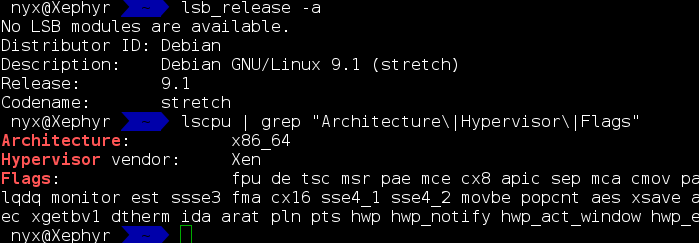
\includegraphics[width=0.75\textwidth]{Figures/sistema-base.png}
    \end{center}
  	\caption{Información del Sistema Base.}
    \label{sistema-base}
\end{figure}

\index{Ejecutar Código}
Como se presenta en la figura \ref{sistema-base}, el sistema base para el desarrollo de este trabajo de titulación utiliza Xen instalado con Debian Stretch (9.1)\footnote{Como el sistema de Dom0} instalado en un LVM con el nombre del grupo de volúmenes ''Xephyr-VG''. Originalmente se tenía planificado trabajar con Debian Jessie (8.x) debido que esa era la versión estable al momento de la instalación, sin embargo luego se optó por la actualización a la versión beta de Debian del momento (Debian Stretch). En resumen los pasos realizados fueron:
\lstset{language=Bash}
\begin{enumerate}
	\item Instalación Limpia de Debian 8 con un LVM.
    	\begin{description}
    		\item[Volumen Físico:] /dev/sda8 310g 
            \item[Grupo de Volúmenes:] Xephyr-VG 310g
            \item[Volúmenes Lógicos:] Originalmente 4 (se agrega 2 por cada nueva máquina virtual -- uno para su disco y otro para su área de intercambio).
            \begin{description}
            	\item[Xephyr-Dom0] Xephyr-VG 30g
                \item[Xephyr-IMG-Repo] Xephyr-VG 20g
                \item[Xephyr-ISO-Repo] Xephyr-VG 20g
                \item[Xephyr-Swap] Xephyr-VG 4g
            \end{description}
    	\end{description}
    \item Actualizar la instalación de Debian 8.
    	\begin{lstlisting}
	apt update
	apt upgrade
	apt dist-upgrade
	reboot
        \end{lstlisting}
    \item Actualizar Debian 8 a Debian 9.
        \begin{lstlisting}[breaklines=true]
	sed -i 's/jessie/stretch/g' /etc/apt/sources.list
	apt update
	apt upgrade
	reboot
        \end{lstlisting}
    \item Instalación de las Herramientas de Trabajo
        \begin{lstlisting}
	apt install tmux vim zsh
        \end{lstlisting}
    \item Instalación y Configuración de Hipervisor Xen
		\begin{lstlisting}[breaklines=true]
	apt install xen-hypervisor
	dpkg-divert --divert /etc/grub.d/08_linux_xen --rename /etc/grub.d/20_linux_xen
	update-grub
	cat > /etc/network/interfaces.d/xenbr << EOF

	auto xenbr0
	iface xenbr0 inet static
		address 10.10.10.1
		netmask 255.255.255.0
		bridge_ports wlan0

	#other possibly useful options in a
	#	virtualized environment
		#bridge_stp off		# disable
		#		Spanning Tree Protocol
		#bridge_waitport 0	# no delay
		#		before a port becomes
		#		available
		#bridge_fd 0		# no forwarding
		#		delay

	## configure a (separate) bridge for
	#	the DomUs without giving Dom0 an
	#	IP on it
	#auto xenbr1
	#iface xenbr1 inet manual
	#   bridge_ports eth1

	EOF

	reboot
		\end{lstlisting}
	\item Instalación de Herramientas de Xen
		\begin{lstlisting}
	apt install xen-tools xen-utils
		\end{lstlisting}
    \item Instalación de Herramientas de Desarrollo para Python 3
    	\begin{lstlisting}
	apt install python3 python3-virtualenv python3-pip
    	\end{lstlisting}
    \item Instalación de Servidores
    	\begin{lstlisting}[breaklines=true]
	apt install nginx-full postgresql mongodb redis-server gitweb fcgiwrap
    	\end{lstlisting}
    \item Instalación de otras dependencias
        %  % TODO: Look for other possible dependencies?
    	\begin{lstlisting}
	apt install libffi-dev
    	\end{lstlisting}
    \item Instalación de IDEs en /opt. Se descargaron los respectivos .tar\textit{.xx} y se los descomprimió en /opt con un comando similar al siguiente:
    	\begin{lstlisting}[breaklines=true]
	tar -axvf nombre.tar.xx -C /opt/ruta/raiz/donde/descomprimir
    	\end{lstlisting}
    \begin{enumerate}
    	\item PyCharm (Community o Professional Edition\footnote{Se ocupó la versión profesional, en parte por elbuen soporte para el desarrollo con Django) con una licencia estudiantil que actualmente que permite solicitar y renovar año tras año con un correo institucional})
        \item DBeaver (Community o Enterprise Edition\footnote{Históricamente siempre han sido gratis ambas versiones con la diferencia que Enterprise Edition no es completamente software libre y agrega soporte para bases de datos no relacionales. Se ocupó la versión Enterprise, de las últimas ofertas gratis antes de que se convierta en un producto de pago, por el mismo motivo de requerir soporte para bases de datos NoSQL como MongoDB y Redis.})
    \end{enumerate}
\end{enumerate}

Estos pasos de instalación se basaron en la guía de instalación de Xen publicado en el wiki del proyecto de Debian \citep{Debian-Wiki-Xen}.

Para dar conexiones hacia el exterior de las maquinas virtuales, se necesita activar una regla NAT en el cortafuego IPTables:

\begin{lstlisting}[breaklines=true]
	iptables -t nat -A POSTROUTING -o wlan0 -j MASQUERADE
\end{lstlisting}

\index{Controlar Versiones de Código} \index{Persistir Código}
\subsubsection{Servidor Local de Git}
Para gestionar versiones de código escrito y facilitar la integración con sistemas externos y el sistema de virtualización, se levantó un servidor sencillo de Git. La instalacion del mismo se documenta en el Anexo \ref{AnexoC}.

\index{Persistir Código} \index{Controlar Versiones de Código}
\subsubsection{Git Server HTTP Endpoint}
Para recibir llamadas HTTP y convertirlas en sus respectivos objetos, en un repositorio de Git se creó un miniservicio que realiza esta tarea, basado en la misma aplicación de autenticación que utiliza EduNube:
\begin{lstlisting}
pipenv --three
pipenv install django six psycopg2 PyJWT bcrypt ipython \
	requests
pipenv run django-admin startproject GitServerHTTPEndpoint .
# Configurar Base de Datos, Reutilizar authApp de EduNube, \
#	migrar la base de datos, Crear un superusuario
rsync -av --progress ~/EduNube/authApp \
	~/GitServerHTTPEndpoint/
vim GitServerHTTPEndpoint/settings.py
pipenv run python manage.py makemigrations authApp
pipenv run python manage.py migrate
pipenv run python manage.py createsuperuser

pipenv run python manage.py runserver 8002
# crear un api token para GitEDU

pipenv run python manage.py startapp apiApp

pipenv lock --requirements | awk '{print $1}' > \
	requirements.txt
\end{lstlisting}

Se puede encontrar el repositorio para este servicio en \url{https://gitlab.com/nishedcob/GitServerHTTPEndpoint}.

\paragraph{Tokens de Autenticación}
Para el uso del API del servicio de GitServerHTTPEndpoint, se emite tokens mediante una interfaz CRUD, construida con formularios de Django. Estos API tokens son construidos bajo el estandar JWT o JSON Web Tokens donde el servidor (servicio de Django) generar una llave secreta (mediante la función generar sal de bcrypt) y con ello se cifra los  datos sobre el cliente con el fin de poder validar la identidad del mismo mediante el API token sin que el cliente pueda modificar los datos de su API token. El mismo esquema de autenticación para el API se utiliza con el servicio de EduNube. El acceso al mismo se puede encontrar en la url \url{http://10.10.10.1:8020/auth/tokens} y acceder con cualquier cuenta de superusuario para la creación, lectura, actualización y eliminación de los API Tokens.

\paragraph{API externa}
Los URLs del API de GitServerHTTPEndpoint toman la forma general de: 
\texttt{/api/<tipo\_de\_objeto>/<accion>/<ruta/de/objeto>}\\
donde los tipos de objetos posibles son:
\begin{itemize}
	\item \texttt{ns} para los Namespace
    \item \texttt{repo} para Repositorios y
    \item \texttt{file} para Archivos
\end{itemize}
acciones posibles son:
\begin{itemize}
	\item \texttt{create} para crear,
	\item \texttt{edit} para editar y
    \item Para el caso de los archivos, no existe un solo \texttt{edit} si no una subclasificacion de:
    \begin{itemize}
    	\item \texttt{edit/mv}
        para alterar la ruta de un archivo y 
        \item \texttt{edit/contents}
        para alterar los contenidos de un archivo.
    \end{itemize}
\end{itemize}

Los URIs del API que operan sobre Namespace, solo aceptan un namespace de parámetro con un slash de delimitador final por ejemplo: \\
\texttt{/api/ns/create/nearley/}

Los URIs del API que operan sobre los repositorios requieren de los parámetros: un namespace y un repositorio igual con un slash de delimitador final por ejemplo: \\
\texttt{/api/repo/create/nearley/GitEDU/}

Los URIs del API que operan sobre archivos toman de parámetros un namespace, un repositorio y una ruta de archivos que puede llevar cualquier número de slash para indicar los directorios dentro del repositorio selecionado, pero la misma ruta no puede terminar en un slash, por ejemplo: \\
\texttt{/api/file/create/nearley/GitEDU/despliegue/Readme.md}

Un cliente ejemplar de todo el API, se puede encontrar con el nombre \\
\texttt{example\_client.py} dentro de la raíz del proyecto.

\index{Sincronizar Notas por LTI} \index{Autenticación LTI}
\subsection{Ambiente Virtual de LMS \index{LMS} (Moodle)}
\label{instalacion-moodle}
Originalmente se planteó trabajar con un LMS como una máquina virtual de Xen, pero con el tiempo, se ha vio la necesidad de consumir todos los servicios posibles de una forma mas liviana y por lo tanto aunque se incluye por este medio la instalación de Moodle en una máquina virtual de Xen, detallado en el Anexo \ref{AnexoC}, al final se optó por un levantamiento del mismo en Docker. El levantamento de Moodle en Docker se documenta en el capítulo \ref{capitulo6} de Despliegue.

\index{Persistir Código} \index{Controlar Versiones de Código}
\subsection{Servidor de Git (GitLab CE)}
Originalmente se planteó trabajar con GitLab Community Edition como una máquina virtual de Xen, pero con el tiempo, se ha vio la necesidad de consumir todos los servicios posibles de una forma más liviana al final se optó por un levantamiento del mismo en Docker. Sin embargo en este documento se incluye la instalación de la primera opción en una máquina virtual de Xen, detallado en el Anexo \ref{AnexoC}, . El levantamento de GitLab en Docker se documenta en el capítulo \ref{capitulo6} de Despliegue.

\index{Ejecutar Código}
\subsection{Servidor de Virtualización}
Para la ejecución de código se consideró necesario la virtualización. La ejecución puramente nativa de código daría mayor grado de ataques al servidor físico además de no brindar de una flexibilidad necesaria para sostener una gran variedad de usuarios y necesidades.

\index{Ejecutar Código}
\subsubsection{Comparación de Hipervisores}
Para la selección de una tecnología de virtualización, se ha considerado conveniente realizar el siguiente cuadro comparativo, en base a una valoración de características de cada ecosistema de hipervisor generando una calificación ponderada de las mismas y poder llegar objetivamente al mejor hipervisor a ser implementado en el presente proyecto.

\begin{table}
	\centering
	\begin{tabular}{|l|r|}
    	\hline
		\textbf{Característica} & \textbf{Peso} \\
        \hline
        \textit{Rendimiento} & 10 \\
        \textit{Seguridad} & 10 \\
        \textit{Facilidad de Uso (CLI)} & 10 \\
        \textit{Facilidad de Uso (GUI)} & 5 \\
        \textit{Facilidad de Uso (WUI)} & 5 \\
        \textit{Facilidad de Instalación} & 5 \\
        \textit{Facilidad de Mantenimiento} & 5 \\
        \textit{Experiencia Personal del Autor} & 10 \\
        \hline
        \textbf{Total de Pesos} & 60 \\
        \hline
	\end{tabular}
    \caption{Pesos de las Características de Comparación para Hipervisores Considerados}
    \label{tab:hipervisor-compar-pesos}
\index{Ejecutar Código}
\end{table}

El cuadro \ref{tab:hipervisor-compar-pesos} presenta los pesos que se asignaron a cada categoría de la comparación, para poder realizar un promedio ponderado de las valoraciones con mayor peso en las categorías que se consideraban más importantes. Las características consideradas son:
\begin{description}
	\item[Rendimiento], indica la máxima eficiencia que puede llegar a tener la virtualización con esta tecnología.
    \item[Seguridad], indica el nivel de aislamiento y mitigación de riesgo que se considera los usuarios virtualizados frente la máquina host.
    \item[Facilidad de Uso (CLI)], la facilidad en utilizar el hipervisor desde línea de comandos (terminal).
    \item[Facilidad de Uso (GUI)], la facilidad en utilizar el hipervisor desde una aplicación de escritorio gráfico.
    \item[Facilidad de Uso (WUI)], la facilidad en utilizar el hipervisor desde la plataforma web.
    \item[Facilidad de Instalación], la facilidad para instalar el hipervisor y realizar la configuración inicial para que empiece a funcionar.
    \item[Facilidad de Mantenimiento], la facilidad para actualizar, utilizar y mantener el hipervisor.
    \item[Experiencia Personal del Autor], la opinión que tiene el autor del hipervisor después de años de uso y experimentación en estas tecnologías.
\end{description}
Se ha considerado con mayor importancia el Rendimiento y la Seguridad como necesidades del presente proyecto. La Facilidad de Uso desde la Línea de Comandos y la Experiencia Personal del Autor también se ha considerado importante para que se pueda implementar de forma mas concisa, rápida y precisa la tecnología de virtualización elegida. La Facilidad de Uso tanto Gráfica como Web en adición a la complejidad de la instalación y mantenimiento se considera importantes pero menos relevantes, debido a que son características de menor impacto para el desarrollo actual y a largo plazo es donde tienen mayor impacto se puede implementar otra solución más adecuada frente a estos temas si es necesario. 

\begin{table}
	\centering
	\begin{tabular}{|p{1.85cm}|p{2.25cm}|p{1.8cm}|p{1.7cm}|p{1.7cm}|p{1.7cm}|}
    	\hline
		\textbf{Hipervisor} & \textbf{Rendimiento} & \textbf{Seguridad} & \textbf{Facilidad de Uso (CLI)} & \textbf{Facilidad de Uso (GUI)} & \textbf{Facilidad de Uso (WUI)} \\
        \hline
        \textit{Xen} & 4 & 5 & 4 & 3 & 2 \\
        \hline
        \textit{KVM} & 3 & 5 & 4 & 3 & 3 \\
        \hline
        \textit{Docker} & 5 & 3 & 5 & 3 & 4 \\
        \hline
	\end{tabular}
    \caption{Características de Comparación I: Hipervisores Considerados}
\index{Ejecutar Código}
    \label{tab:hipervisor-compar-i}
\end{table}

\begin{table}
	\centering
	\begin{tabular}{|p{1.85cm}|p{2.2cm}|p{3.0cm}|p{1.9cm}|}
    	\hline
		\textbf{Hipervisor} & \textbf{Facilidad de Instalación} & \textbf{Facilidad de Mantenimiento} & \textbf{Experiencia Personal del Autor} \\
        \hline
        \textit{Xen} & 3 & 2 & 4 \\
        \hline
        \textit{KVM} & 4 & 2 & 2 \\
        \hline
        \textit{Docker} & 5 & 4 & 4 \\
        \hline
	\end{tabular}
    \caption{Características de Comparación II: Hipervisores Considerados}
\index{Ejecutar Código}
    \label{tab:hipervisor-compar-ii}
\end{table}

% TODO: Correccion de la Maria del Carmen "caracteristicas consideradas"?
En los cuadros \ref{tab:hipervisor-compar-i} y \ref{tab:hipervisor-compar-ii} se presenta las características consideras y un puntaje relativo (sobre 5) dado a cada una de estos de acuerdo a investigaciones, experiencias y opiniones del autor. A continuación se explica el porqué de las valoraciones:
\begin{description}
	\item[Xen] como un hipervisor de tipo 1 cuenta con un rendimiento muy alto, especialmente cuando se lo considera la paravirtualización que también soporta sistemas operativos modificados, casi a un nivel nativo. Este hipervisor logra virtualizar todas las capas de un sistema operativo, desde su núcleo hasta el espacio de los usuarios, pero al mismo tiempo dispone de un modelo de seguridad muy bueno. Tiene falla en las herramientas de administración, de los cuales hay muy pocas que están actualizadas. La mejor herramienta de administración es en la Línea de Comandos. Sus cambios frecuentes y documentación desactualizada son un problema para la instalación y mantenimiento. Sin embargo, la experiencia del autor con esta tecnología ha sido muy positiva.
    \item[KVM] como un hipervisor de tipo uno y medio tiene un nivel más alto que Xen pero no dispone del mismo nivel de rendimiento que ofrece ni la paravirtualización. Aunque es de más alto nivel, se ha xonsiderado otros pasos adicionales para alcanzar un nivel de seguridad equivalente al de Xen. Para su administración cuenta con herramientas muy similares a los de Xen, pero su alto nivel de integración con el API de Libvirt hace que cuente con mejores interfaces para su manejo web. Posiblemente por desconocimiento de las posibilidades para mejorar el rendimiento que se puede aplicar, el autor no ha tenido una experiencia muy positiva con la aplicación de esta tecnología de virtualización.
    \item[Docker] como un hipervisor de ''tipo tres'' es de muy alto nivel y dispone de una seguridad mucho menor al tener menor aislamiento entre el sistema que provee la virtualización y la virtualizada. Docker tiene mejor rendimiento ya que se virtualiza solo los niveles más altos de un sistema operativo y las aplicaciones que se encuentran por encima. Su técnica de contenerización como un tipo de virtualización, puede dar un mejor rendimiento que la paravirtualización. Se considera muy buena las interfaces para utilizar Docker, tanto a nivel de terminal como a nivel Web, por el hecho de que Docker es una tecnología que aún es nueva y que esta en auge. Esto promueve a una gran cantidad de personas en contribuir continuamente con mejoras. La instalación y mantenimiento de Docker es muy sencilla en cualquier plataforma. Debido a su sencillez, alto rendimiento, funcionalidad y utilidad, el autor ha tenido una buena experiencia con el uso de esta tecnología de virtualización. 
\end{description}

Para calcular los pesos promedio de forma ponderada se aplica la fórmula que se encuentra en la figura \ref{fig:hipervisor-calif-equ}. Las calificaciones promedias se reflejan en el cuadro \ref{tab:hipervisor-compar-promed}. Como se puede observar en el mismo cuadro, frente a los criterios previamente establecidos, Docker se puede considerar la mejor tecnología de virtualización en el proyecto actual con un puntaje de $4.167$, con medio punto más que su competencia mas cercana Xen, $3.667$ y $\frac{5}{6}$ de un punto más que KVM, $3.333$, que está en último lugar.

\begin{figure}
	\[
		Promedio = \sum_{c = [Categorías]} CalificaciónCatagoria_c * \left ( \frac{PesoCatagoria_c}{TotalPesos} \right )
	\]
	\caption{Ecuación para calcular los promedios ponderados en base a pesos para los hipervisores comparados}
    \label{fig:hipervisor-calif-equ}
\index{Ejecutar Código}
\end{figure}

\begin{table}
	\centering
	\begin{tabular}{|l|r|}
    	\hline
		\textbf{Hipervisor} & \textbf{Calificación Promedio Ponderado} \\
        \hline
        \textit{Xen} & 3.667 \\
        \hline
        \textit{KVM} & 3.333 \\
        \hline
        \textit{Docker} & 4.167 \\
        \hline
	\end{tabular}
    \caption{Calificaciones Promediados Ponderadas para la Comparación de los Hipervisores}
    \label{tab:hipervisor-compar-promed}
\index{Ejecutar Código}
\end{table}

\index{Hipervisor} \index{Virtualización} \index{Contenedor}
\subsubsection{Servidor de Virtualización Virtualizado}
Frente las desventajas/problemas que tiene Docker, se ha elegido a Kubernetes como una tecnología complementaria para la orquestación con la nube, y brindar a futuro una mayor independencia a la plataforma EduNube frente a cualquier hipervisor en particular. El otro candidato considerado para esta capa intermedia de orquestación de nube, entre EduNube y los respectivos hipervisores que se puede utilizar, fue OpenStack debido a que es una solución muy completa para el problema actual con más características que de los Kubernetes, pero el mismo, por su gran lista de características es muy pesado y no entraría adecuadamente en la infrastructura actual de la Universidad Técnica Particular de Loja, entonces para ofrecer una solución que cumpla con el contexto actual de la universidad, los Kubernetes ofrecen una buena alternativa que, aunque sea relativamente liviana, ofrece las características necesarias para implementar una solución de ejecucion que sea eficaz y eficiente en la infrastructura actual. Kubernetes ocupa una arquitectura cliente-servidor, motivo por el cual se lo instala en dos fases; primero el cliente y después de forma virtualizada, para ayudar a mitigar algunos de los riesgos asociados con Docker, el servidor. 

\index{Kubernetes}
\paragraph{Kubernetes}
La instalación y uso de Kubernetes se encuentra en el Anexo \ref{AnexoC}.

\index{Docker}
\subsection{Plantillas de Máquinas Virtuales (Docker)}
Para la ejecución de código en Docker, es necesario tener un contenedor de Docker que cumpla con las dependencias requeridas al momento de la ejecución. Los contenedores están basados en Debian y en Alpine Linux.

\subsubsection{Sistema Operativo: Debian GNU/Linux}
Se considera Debian como una buena base para los contenedores debido a que es bastante conocido, estable, seguro y tiene una amplitd de paquetes que se pueden instalar directamente desde sus repositorios oficiales.

\subsubsection{Sistema Operativo: Alpine GNU/Linux}
Alpine Linux es muy utilizado en el mundo de los contenedores (por ejemplo con Docker) y en la nube en general porque es un sistema operativo minimalista que lleva menor peso. Aquí tiene el mismo fin, aunque aveces es mas complicado de manejar y configurar, puede que valga la pena para entornos de producción que necesitan optimizar el uso de sus recursos.

\index{Docker|(}
\subsubsection{Tipo de Contenedor: Shell-Executor}
El tipo de contenedor ''Shell-Executor'' es para ejecutar comandos dentro de un contenedor con el shell ''sh'' y forma la base para los otros tipos de contenedores. Tanto en Debian como en Alpine no hay necesidad de instalar más paquetes, ya que la imagen por defecto viene con todo lo necesario. Lo que si se tiene que definir para estos contenedores es un usuario menos privilegiado con el cual se ejecuta los comandos/código dentro del contenedor y una ubicación, un volumen desde el punto de vista de Docker, donde se puede enviar el código a ser ejecutado. La diferencia entre la implementación tanto en Debian y Alpine es la creación de un usuario con menos privilegios en adición a la imagen base que se toma. La implementacion del mismo se puede encontrar en el Anexo \ref{AnexoD}.

\subsubsection{Tipo de Contenedor: Python3-Executor}
El tipo de contenedor ''Python3-Executor'' es para ejecutar comandos de shell en adición a código de Python 3. Se extiende de los contenedores definidos para el ''Shell-Executor'' para proveer de la funcionalidad de ejecutar comandos en un shell. El punto de entrada de ejecución es el archivo ''main.py'' a nivel raíz del repositorio. Tanto Debian como Alpine requieren de la instalación de Python 3, ya que la versión de Python por defecto es 2.7 que actualmente debería considerarsela prácticamente obsoleta. Docker requiere que se vuelva a definir los volúmenes y para la adecuada ejecución del código también se define la ubicación inicial de ejecución como el mismo volumen que se monta desde un sistema de ficheros externo al contenedor. La implementacion del mismo se puede encontrar en el Anexo \ref{AnexoD}.

\subsubsection{Tipo de Contenedor: PostgreSQL-Executor}
El tipo de contenedor ''PostgreSQL-Executor'' es para ejecutar comandos de shell en referencia a SQL de PostgreSQL. Se extiende de los contenedores definidos para el ''Shell-Executor'' para proveer la funcionalidad de ejecutar comandos en un shell. El archivo ''init.sql'' se ejecuta primero y por lo tanto puede ser utilizado para generar y llenar la base de datos. El archivo ''main.sql'' se ejecuta después y por lo tanto podría ser útil para ejecutar comandos SQL definidos por el usuario. Tanto Debian como Alpine requieren de la instalación de PostgreSQL, tanto cliente como servidor. Docker requiere que se vuelva a definir los volúmenes y para la adecuada ejecución del código, también se define la ubicación inicial de ejecución como el mismo volumen que se monta desde un sistema de ficheros externo al contenedor. La implementacion del mismo se puede encontrar en el Anexo \ref{AnexoD}.
\index{Docker|)}

\section{GitEDU}

La gestión de dependencias del sistema GitEdu se maneja con un entorno virtual y el gestor de paquetes de python pip. El siguiente es un script de bash diseñado para detectar si es que existe el entorno virtual (lo crea en caso que no exista) y después instala los requerimientos faltantes como son especificados en un archivo aparte ''requirements.txt'' en el que se encuentran las librerías necesarias y sus versiones.

\begin{lstlisting}

# run with `source activate.sh` 
if [ ! -d env ]; then
	virtualenv --python=python3 env
fi
source env/bin/activate
pip3 install -r requirements.txt

\end{lstlisting}

El script anterior se ejecuta desde el raíz del repositorio con el comando:

\begin{lstlisting}
source activate.sh
\end{lstlisting}

Con el entorno creado y activado se puede proceder a instalar cualquier dependencia necesaria que no ha sido instalado previamente:

\begin{lstlisting}
pip install <nombre_dependencia>
\end{lstlisting}

Para el presente proyecto se instalaron las siguientes dependencias:
\begin{itemize}
	\item Django (1.10.6) como framework para el desarrollo del backend.
    \item Psycopg2 (2.7.1) como librería para conectarse a bases de datos PostgreSQL.
    \item Python-GitLab (0.20) como librería para consumir el API de GitLab.
    \item ipython (6.1.0) como interprete interactivo de Python para hacer pruebas en el curso del desarrollo.
\end{itemize}

Con las dependencias instaladas o con cada cambio que se realice de las dependencias, se ejecuta el siguiente comando para actualizar la lista de las mismas:

\begin{lstlisting}
pip freeze > requirements.txt
\end{lstlisting}

Se inicia el proyecto de Django con el comando:

\begin{lstlisting}
django-admin startproject GitEdu
\end{lstlisting}

También antes de iniciar el desarrollo debe estar configurada la base de datos para proceder a ocuparla.  Esto se documenta en el Anexo \ref{AnexoD}.

Ahora se puede migrar las tablas iniciales de Django:
\begin{lstlisting}
cd GitEDU
python manage.py makemigrations
python manage.py migrate
\end{lstlisting}

También creamos un superusuario de Django para temas administrativos:
\begin{lstlisting}
python manage.py createsuperuser
\end{lstlisting}

\index{Editar Código}
También se puede crear el app inicial (para lógica del editor de código):
\begin{lstlisting}
python manage.py startapp ideApp
\end{lstlisting}

Y de paso se lo agrega a INSTALLED\_APPS una linea 'ideApp' en el settings.py para que las tablas definidos a futuro en models.py también se migren con los demás migraciones.

Para resolver un problema de zonas de tiempo, se ha desactivado esta característica de Django con la siguiente línea en el settings.py:
\lstset{language=Python}
\begin{lstlisting}
USE_TZ = False
\end{lstlisting}
\lstset{language=Bash}

La creacioón de la base de datos NoSQL y su configuración con Django se encuentra en el Anexo \ref{AnexoD}.

\subsubsection{Automatización del Levantamiento del Servicios / DevStack}
Para el manejo de dependencias, inicialmente se lo manejó unicamente con Pip y Virtualenv hasta que se descubrió otra herramienta que combina la funcionalidad de ambos en un solo commando: \texttt{pipenv}. El mismo agrega funcionalidades adicionales como validacion del ambiente (sistema operativo / arquitectura / versión exacta de Python) y validación de paquetes (mediante sus hash SHA256). Es por ello que se vio la importancia en cambiar la modalidad con que se llevaba las dependencias del proyecto, aunque también se sigue apoyando el método anterior para quienes no realizan la instalacion de pipenv con pip como root.

Para el fácil levantamiento del DevStack, se realizó dos scripts, de los cuales cada uno detecta la presencia de pipenv para utilizarlo si existe o no existe ocupar la modalidad clásica de virtualenv con pip para gestionar las dependencias. Lo que diferencia los dos scripts es que uno, después de validar/instalar y activar el entorno, ejecuta el servidor en el puerto designado para producción (\texttt{runserver}) mientras que el otro (\texttt{runshell}) abre el shell de Django después de adecuar el entorno.

\subsection{Autenticación Clásica}

Primero se crea una nueva aplicación para autenticación clásica:
\begin{lstlisting}
python manage.py startapp authApp
\end{lstlisting}

Y de paso se lo agrega a INSTALLED\_APPS en una línea 'authApp' en el settings.py para que las tablas definidos a futuro en models.py también se migren con las demás migraciones.

Para la implementación de autenticación clásica, se reutilizó el módulo con el mismo propósito del proyecto anterior GitEduERP. A esta se aumentó la funcionalidad adicional, que es que desde el settings se pueda activar o desactivar la funcionalidad de permitir a los usuarios registrarse a través del atributo ENABLE\_REGISTRATION. 

Para el registro de usuarios, se considera que solo debe permitirse (en caso de que sea habilitado por la administración) el registro de estudiantes y docentes pero no de administradores, motivo por el cual se ha considerado duplicar los formularios de registro y ofrecer uno para estudiantes y otro para docentes. Los mismos se pueden habilitar y deshabilitar con los atributos ENABLE\_STUDENT\_REGISTRATION y ENABLE\_TEACHER\_REGISTRATION respectivamente.

\index{Autenticación LTI}
\subsection{Autenticación por LTI}
Se documenta el proceso de levantamiento de autenticación por LTI en el Anexo \ref{AnexoD}.

\subsubsection{Validación}

Se levanta la aplicación (en \url{http://localhost:8000/} con:
\begin{lstlisting}
python manage.py runserver
\end{lstlisting}
La máquina virtual de Moodle también debe estar levantada para navegar a \url{http://10.10.10.10/}, iniciar sesión como administrador, e ir a la parte administrativa, a la pestaña de ''development'', seleccionar ''debugging'', y poner ''debug messages'' a nivel ''developer''. Ahora podemos volver a la parte de administración, volver a seleccionar la pestaña de ''development'' y crear un curso de prueba. Vamos a crear un curso pequeño (10 MB) con el nombre corto ''Prog\_I'' y nombre largo / descripción ''Introducción a la Programación''. Una vez que se carga el curso, activamos el modo de editar y agregamos una actividad externa.

Se da un nombre a la actividad, en este caso ''Prueba 1 Programación''. La mejor forma de poder reutilizar la herramienta externa en varias actividades es de crear una herramienta ''Preconfigurada''. Las opciones elegidas para la misma fueron los siguientes:
\begin{description}
	\item[Nombre] GitEdu
    \item[URL] \url{http://localhost:8000/lti/launch}
    \item[Descripción] Edit Code Online
    \item[Llave de Consumidor] GitEduLMS\_Playground
    \item[Secreto Compartido] b2e0158c3cb4ddb0202d
    \item[Parámetros Adicionales] lo dejamos en blanco
    \item[Contenedor de Lanzamiento] Nueva ventana
    \item[Compartir Nombre] Siempre
    \item[Compartir Correo Electrónico] Siempre
    \item[Aceptar Notas] Siempre
\end{description}
Con la herramienta preconfigurada realizada, se puede seleccionarlo así no mas para completar la integración. Donde se creó la actividad debe haber un enlace con el nombre del mismo, en este caso ''Prueba 1 Programación''. Al abrir el enlace se debe llevar a la aplicación con los siguiente puntos interesantes:
\begin{enumerate}
	\item se encuentra autenticado con el mismo usuario de Moodle (incluyendo sus roles como ''administrador'', ''instructor'', ''estudiante'', etc\ldots{})
    \item hay contexto de:
    \begin{enumerate}
    	\item el curso de origen de Moodle
        \item la actividad de origen de Moodle (no es contexto completo, un problema que se tendrá que resolver en el curso del desarrollo)
        \item la llave de consumidor ocupada
    \end{enumerate}
\end{enumerate}

Si, dentro del mismo curso creamos una segunda actividad con todo lo mismo, pero solo cambiando el nombre a ''Prueba 2 Programación'', se identifica que sí se logra distinguir entre actividades.

\subsection{Integración de dos esquemas de autenticación}
Los dos schemas de autenticación implementados, sea la forma clásica con nombre de usuario y contraseña correspondiente o por LTI \index{LTI} donde una aplicación externa autentica un usuario autenticado previamente por el mismo, tienen el mismo fin de permitir que el sistema conozca quién esta accediendo al sistema para actuar con el comportamiento adecuado y en base a ello proveer seguridad y funcionalidad a todos los usuarios según su rol.

Se propone tres tablas (EquivalentUser, AuthenticationType, UserAuthentication) en la base de datos expresados como modelos de Django, los mismos que se encargaran de generar las tablas adecuadas en la base de datos a través de su ORM interno.

La tabla EquivalentUser relaciona a los usuarios autenticados de forma clásica con usuarios autenticados por LTI \index {LTI} (porque por cada método de autenticación se crea un nuevo usuario para su uso interno) con el fin de permitir relacionar distintos usuarios dentro del sistema quienes representan el mismo individuo natural. La idea es por ejemplo, si un docente se autentica por LTI \index{LTI} y también por usuario y contraseña, para el sistema esta ocupando dos usuarios diferentes pero para el docente esta accediendo el mismo sistema y por lo tanto el comportamiento del sistema, sin tomar en cuenta como se autentica, debe ser igual y debe tener acceso a los mismos contenidos. La tabla AuthenticationType es un catálogo de las formas de autenticación que suporta el sistema y por su naturaleza de catálogo se llena con las migraciones. Y finalmente la tabla UserAuthentication documenta el tipo de autenticación asociada con un usuario para dar el contexto al sistema que necesita para manejar distintos datos de los diferentes tipos de usuarios. La migracion escrita a mano para llenar la tabla AuthenticationType se puede encontrar en el Anexo \ref{AnexoD}.

\subsection{Accesibilidad a Datos de Autenticación de LTI}
Las vistas y settings definidas para exponer datos de la autenticacion por LTI se presenta en el Anexo\ref{AnexoD}.

\index{Calificar Código}
\subsection{Establecer un Modelo de Base de Datos}
Para empezar con el desarrollo de la parte fuerte del sistema GitEDU, es importante considerar su modelo de base de datos preliminar. La parte más importante de ello son las tablas o entidades y las relaciones entre las mismas. Para esto se ha considerado 3 grupos de funcionalidades importantes:
\begin{enumerate}
	\item El aspecto social y con ello varios roles con los que se puede manejar a los usuarios dentro del sistema. Esto se representa con el app 'socialApp'.
    \item El aspecto académico, se refiere a cómo se llevan las materias académicas dentro del sistema. Esto se representa con el app 'academicApp'.
    \item El aspecto de las calificaciones y con ello la forma en que se llevan las calificaciones que los estudiantes obtienen en las materias. Este aspecto es muy relacionado con el tema anterior de la parte académica y la línea que las divide es un poco subjetiva ya que por lo mismo hecho no se ha optado por la creación de tablas adicionales para separar estos dos aspectos, de todas maneras donde ha sido posible, se ha realizado la división. Este aspecto se representa con el app 'gradesApp'. 
\end{enumerate}

\begin{lstlisting}
python manage.py startapp socialApp
python manage.py startapp academicApp
python manage.py startapp gradesApp
\end{lstlisting}

Cada una de las anteriores aplicaciones han sido agregadas al INSTALLED\_APPS del settings para que Django reconozca la necesidad de tomar en cuenta los modelos de cada uno.

Los modelos iniciales del socialApp solo definen distintos roles sociales dentro del sistema y ocupan cuatro tablas:
\begin{enumerate}
	\item Person
	\item Student
	\item Teacher
	\item Administrator
\end{enumerate}
Se esta tomando en cuenta que la tabla de usuarios de Django ya lleva por defecto muchos detalles de los usuarios como sus nombres y apellidos, por lo tanto no hay necesidad de replicar estos datos. Esta jerarquía de clases viene a ser la infraestructura necesaria para definir a cada uno de los usuarios en caso de que sea necesario.

El modelo inicial de academicApp permite a los docentes y administradores definir las materias ofrecidas (con paralelos y metadatos como categoría del componente), ya sean los mismos docentes o sus estudiantes, adicionalmente de proveer de la infraestructura de datos necesaria para que un docente pueda definir su libreta de calificaciones a una materia, en base a un sistema relativo o un sistema de promedios ponderados (el sistema puede calcular en base al sistema relativo). Esto involucra nueve tablas en la base de datos:
\begin{enumerate}
  \item ClassSubject
  \item Course
  \item Section
  \item Classroom
  \item ClassroomTeacher
  \item ClassroomStudent
  \item AcademicCategory
  \item AcademicSubCategory
  \item AcademicAssignment
\end{enumerate}
ClassSubject define el tipo de materia que es, por ejemplo ''Programación'' o ''Base de Datos''. Course define una materia ofrecida, por ejemplo ''Introducción a la Programación''. Section define paralelos ofrecidos de forma general, por ejemplo ''A'', ''B'', ''C'', etc\ldots{} Classroom une las dos tablas anteriores de materia de oferta con paralelo para definir aulas de una materia. ClassroomTeacher define el docente asignado a una aula y el peso que tiene el docente en la nota final de los estudiantes de esta aula. Esto es con un fin de permitir varios docentes con varios pesos dentro de la misma aula emitiendo calificaciones distintas para estudiantes previo a un promedio ponderado del estudiante. ClassroomStudent relaciona estudiantes y aulas. AcademicCategory provee docentes con la oportunidad de disponer de una herramienta para organizar las calificaciones de sus estudiantes en categorías con distintos pesos, por ejemplo ''Exámenes'', ''Deberes'', ''Talleres'', etc\ldots{} AcademicSubCategory viene de la misma linea para permitir subdivisiones de las categorías. AcademicAssignment es la abstracción que se da a los itemes calificadas dentro de una subcatagoría.

El modelo inicial de gradesApp permite persistir notas para cada estudiante bajo el modelo de tres niveles definido previamente de categorías, subcatagorías y itemes de subcatagorías con tres tablas:
\begin{enumerate}
  \item StudentCategoryGrade
  \item StudentSubCategoryGrade
  \item StudentAssignmentGrade
\end{enumerate}

\index{Editar Código}
\subsection{Editor de Código en Linea}
Una de las funcionalidades principales del sistema GitEDU es la capacidad de editar código en linea, la lógica del mismo se realiza en la app 'ideApp'.

Con relación al editor de código en linea, inicialmente se empezó con el trabajo realizado anteriormente en el proyecto GitEduERP y en base al mismo se fue expandiendo las características necesarias en el nuevo sistema. Durante el proceso del desarrollo, se observó una necesidad de desarrollar la mayoría de los componentes desde cero y con el mismo se pudo dar mejoras a la propuesta anterior. A diferencia de GitEduERP, GitEDU espera ofrecer:
\begin{itemize}
  \item Un modelo de permisos más robusto y flexible basado en grupos y usuarios.
  \item Un sistema de persistencia de código el cual ofrece la siguientes características:
    \begin{itemize}
      \item Ser extensible con una programación orientada a objetos.
      \item Manejar versiones de código con un sistema de control de versiones interna llevada por archivos completos
      \item Manejo de jerarquías de sistemas de persistencia para llevar varias sistemas de persistencia en paralelo
    \end{itemize}
   \item Integración con sistemas externas que permiten la ejecución de código.
\end{itemize}

\subsubsection{Modelo de Base de Dato para Editor de Código}
Para el editor de código en linea, es necesaria extender la funcionalidad del modelo de base de datos introducido previamente. Primero se agrega dos entidades a socialApp que representan grupos de personas (usuarios) y membresía dentro de estos mismos grupos con dos tablas:
\begin{enumerate}
\item Group
\item GroupMembership
\end{enumerate}

Dentro de ideApp se crea 4 entidades para representar repositorios (una colección de archivos asociados con un proyecto), el mismo tiene capacidad de un usuario y opcionalmente grupo dueño quien esta encargado de la administración del mismo, archivo mismo que entre sus metadatos esta un lenguaje asociado para ayudar con el manejo del mismo a nivel de editor y a nivel de otros tipo de gestión (como ejecución y compilación), y finalmente membresía de personas y grupos en repositorios con una finalidad de llevar mas adelante un sistema de permisos para restringir acceso y/o otras acciones sobre código por usuarios no autorizados. Estos entidades como tablas en la base de datos son:
\begin{enumerate}
\item Repository
\item File
\item RepositoryPersonMembership
\item RepositoryGroupMembership
\end{enumerate}

\index{Persistir Código}
\subsection{Persistencia de Código}
Para la Persistencia de Código se considera dos backends de persistencia para código con una posibilidad de introducir mas a futuro:
\begin{itemize}
	\item MongoDB como base de datos NoSQL para acceso rápido y recuperación de código persistido de una manera similar a GitEduERP.
    \item GitLab CE, como servidor de Git, manejado con una combinación de la API del mismo y comandos de Git para el manejo de cambios en repositorios.
\end{itemize}

Para el mismo es necesario manejar un API interna estandarizada. La solución propuesta utiliza programación orientado a objetos y un modelo estándar de namespace (como usuario o grupo) que contiene repositorios (que representan proyectos o conjuntos lógicos de archivos) y a su vez contienen dichos archivos. La clase base para estandarización se llama CodePersistenceBackend y se encuentra en generics.py del paquete ideApp.CodePersistenceBackends. Para el manejo de datos dentro del API interna, se estandariza los objetos de datos con las siguientes clases genéricas, las cuales pueden ser sobrescritas en cualquier backend con una finalidad de agregar o cambiar funcionalidad existente. Los mismos también se encuentran en el mismo archivo de generics.py. Estos archivos se puede encontrar en el Apéndice \ref{AnexoF}.

En el settings, hay una necesidad de definir los backends de código y su prioridad:
\lstset{language=Python}
\begin{lstlisting}[breaklines]
CODE_PERSISTENCE_BACKENDS = {
    'mongodb': {
        'use': True,
        'backend': 'ideApp.CodePersistenceBackends.MongoDB.backend.MongoDBCodePersistenceBackend',
        'connection_profiles': NOSQL_DATABASES,
        'connection_profile': 'nosql',
    },
    'gitlab': {
        'use': False,
        'backend': 'ideApp.CodePersistenceBackends.GitLab.backend.GitLabCodePersistenceBackend',
        'connection_profiles': GITLAB_SERVERS,
        'connection_profile': GITLAB_DEFAULT_SERVER,
    }
}

CODE_PERSISTENCE_BACKEND_READ_PREFERENCE = ['mongodb']
CODE_PERSISTENCE_BACKEND_WRITE_OUT = ['mongodb']

MONGODB_CONNECT_TO = 'mongodb'
GITLAB_CONNECT_TO = 'gitlab'
\end{lstlisting}
\lstset{language=Bash}

Por el momento se ha optado por dejar desactivado el backend de GitLab ya que el mismo no esta implementado para ser utilizado.

El gestor de persistencia de código se carga todas las backends de persistencia de código que encuentra en el settings para gestionar las conexiones a las mismas. El mismo esta implementado asimismo como un CodePersistenceBackend para permitir que se puede remplazar fácilmente a futuro si se da el caso. Implementa dos clases de persistencia:
\begin{itemize}
	\item Lectura (read)
	\item Escritura (write) 
\end{itemize}
Y permite para toda operación que se especifique sobre cual grupo se debe realizar la operación. Estos grupos se define en el settings con los variables:
\begin{itemize}
	\item CODE\_PERSISTENCE\_BACKEND\_READ\_PREFERENCE (que también da preferencia del orden en que se debe leer de los backends de persistencia de código)
	\item CODE\_PERSISTENCE\_BACKEND\_WRITE\_OUT que define cuales son y da el orden en que se debe escribir a los backends de persistencia de código.
\end{itemize}
El código completo de este backend se encuentra en el paquete ideApp.CodePersis-tenceBackends en el archivo backend\_mánager.py con el nombre de clase CodePersistenceBackendManager que se puede encontrar en el Apéndice \ref{AnexoF}.

También se define el gestor del backend de persistencia de código en el Settings y el código necesario para cargarlo en el momento adecuado:
\lstset{language=Python}
\begin{lstlisting}[breaklines]
CODE_PERSISTENCE_BACKEND_MANAGER_CLASS = 'ideApp.CodePersistenceBackends.backend_manager.CodePersistenceBackendManager'


def load_code_persistence_backend_manager(load_class=CODE_PERSISTENCE_BACKEND_MANAGER_CLASS):
    try:
        module_path, class_name = load_class.rsplit('.', 1)
    except ValueError:
        msg = "%s doesn't look like a module path" % load_class
        six.reraise(ImportError, ImportError(msg), sys.exc_info()[2])
    mod = importlib.import_module(module_path)
    backend_manager_class = None
    try:
        backend_manager_class = getattr(mod, class_name)
    except AttributeError:
        msg = 'Module "%s" does not define a "%s" attribute/class' % (
            module_path, class_name)
        six.reraise(ImportError, ImportError(msg), sys.exc_info()[2])
    return backend_manager_class()

\end{lstlisting}
\lstset{language=Bash}

\subsubsection{MongoDB}
Para la persistencia de código en MongoDB se define unos modelos de base de datos en Python para su utilización con el ORM PyModm. Se presenta el modelo de base de datos para MongoDB en la figura \ref{nosql-db}.

\begin{figure}
	\begin{center}
    	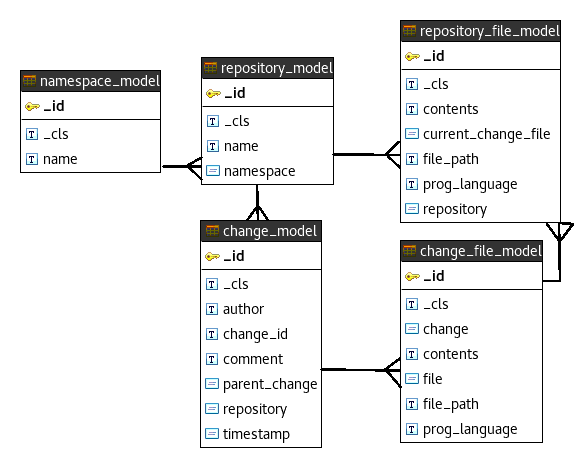
\includegraphics[width=0.75\textwidth]{Figures/nosql-db.png}
    \end{center}
  	\caption{Modelo de Base de Datos en MongoDB.}
    \label{nosql-db}
\end{figure}

El NamespaceModel solo consiste de:
\begin{itemize}
\item el nombre del Namespace
\item el ID que se genera por defecto
\end{itemize}
Esto representa los espacios donde usuarios y grupos pueden crear repositorios. Se considera que los Namespace deben existir de forma única.

El RepositoryModel representa un repositorio y tiene:
\begin{itemize}
\item un nombre
\item permanece a un Namespace
\item el ID que se genera por defecto
\end{itemize}
Cada par de Namespace y Repositorio debe ser una combinación única.

El próximo modelo, RepositoryFileModel, representa un archivo ubicado dentro de un repositorio. Sus atributos son:
\begin{itemize}
\item contenidos del archivo
\item el repositorio a que permanece
\item el lenguaje de programación para que el editor puede cambiar su comportamiento para el lenguaje específico
\item la ubicación del archivo dentro del repositorio incluyendo su nombre
\item un archivo de cambio que representa el estado actual y la última modificación realizada en el mismo, de lo cual se presenta más adelante.
\end{itemize}

El ChangeModel representa un cambio realizado en el repositorio, como los commits de Git. Tiene atributos como:
\begin{itemize}
\item una ID que se lo maneja la aplicación (que viene a ser un hash SHA1, inspirado por Git, de los contenidos y metadatos del mismo cambio)
\item un comentario
\item un autor
\item una estampa de tiempo que tiene tanto la hora como la fecha en que se realizó el cambio
\item el repositorio en que se hizo el cambio
\item una referencia al cambio anterior para que se puede construir una historial de cambios.
\end{itemize}

El ChangeFileModel es como el RepositoryFileModel en que representa archivos, pero en este caso son archivos modificados dentro de un cambio. Por lo tanto lleva los mismos atributos que RepositoryFile solo que en lugar de tener referencias a un repositorio directamente se referencia a un cambio realizado (el cual tiene metadatos como un comentario, autor, cambio previo y momento de modificación) y al archivo del repositorio que modifica (de esta forma puede modificar también la dirección de los archivos quienes no habría otra forma de buscarlos).

Finalmente el TemporaryChangeFileModel no se utiliza actualmente pero como los dos FileModels vistos anteriormente, esta lleva atributos básicos de un archivo. Originalmente se lo planteo para realizar una operación intermedio como la fase del Git Stage en donde se selecciona previo a un commit los cambios que van a estar incluidos dentro del mismo. Pero al final, aunque el modelo de datos esta para suportar varios archivos cambiados dentro de un solo cambio, no esta implementado así. Por temas de tiempo, retraso y alcance, se ha optado por llevar un mini control de versiones de cada archivo dentro de un repositorio, así que en realidad cada cambio en el repositorio solo refleja un archivo cambiado de forma independiente y no hay necesidad para la complejidad del paso intermedio que este modelo representa. 

\index{Controlar Versiones de Código}
\subsubsection{GitLab}
Al settings agregamos las siguientes lineas para configurar la conexión con GitLab:
\lstset{language=Python}
\begin{lstlisting}
GITLAB_DEFAULT_SERVER = '1'

GITLAB_SERVERS = {
    '1': {
        'WITH_TOKEN': True,
        'WITH_CRED': False,
        'API_PROTOCOL': 'http://',
        'API_PORT': '',  # por defecto:
                        # :22 para SSH,
                        # :443 para HTTPS,
                        # :80 para HTTP
        'HOST': '10.10.10.11',
        'SSH_PORT': 22,
        'HTTP_PORT': 80,
        'HTTPS_PORT': 443,
        'USER': "GitEDU",
        'PASSWORD': 'GitEDU2017',
        # expira el 31 de marzo 2018:
        'TOKEN': 'JqMzkgDNvhZ7ofdPa5z5',
        # nunca expira, pero el nivel de 
        # acceso es menor:
        # 'TOKEN': 'TrCfvrdsXzpLFETyc7Q5',  
    }
}
\end{lstlisting}
\lstset{language=Bash}

La implementacion de la conexion al API de GitLab se presenta en el Anexo \ref{AnexoD}.

Aunque originalmente se planifico el uso de GitLab como backend de persistencia de codigo (en repositorios, a diferencia de GitEduERP que ocupó snippets), al final no se ocupó el mismo por cinco razones:
\begin{enumerate}
\item La complejidad del API frente documentacion no tan clara del mismo para el community edition (esta mucho mejor documentado el enterprise edition al cual no se tuvo acceso ni en el ambiente de desarollo ni de produccion) y el tiempo disponible.
\item Un gran inestabilidad del servicio.
\item La falta de recursos en los ambientes de produccion y de desarollo que empeora problemas de estabilidad.
\item La simplicidad de utilizar el sistema de ficheros local directamente con GitWeb para hacer el mismo disponible por HTTP.
\item Realmente frente las necesidades actual del proyecto, con tal que no se necesita exponer el servidor de Git a los usuarios finales, no hay necesidad de un servidor de Git de tanta complejidad como el GitLab.
\end{enumerate}

\subsection{Aspectos Sociales}
Para temas de organización, se ha considerado que aquellos componentes de la aplicación que tienen que ver con interacción social deben existir independientemente de las funcionalidades principales del mismo aplicación. Es con este fin que los componentes del mismo se desarrollaron en un ''app'' distinto 'socialApp'' como fue creada previamente. A futuro se considera el desarollo del mismo para promover interaccion entre estudiantes y tambien otra herramienta de comunicacion e colaboracion entre estudiantes y sus professores que viene a ser un elemento critico para el proceso educativo.

\index{Ejecutar Código}
\section{EduNube}
La gestión de dependencias del sistema EduNube se maneja con un entorno virtual y el gestor de paquetes de python pip. El siguiente es un script de bash diseñado a detectar si es que existe el entorno virtual (lo crea en caso de que no existe) y después instala los requerimientos faltantes como son especificados en un archivo aparte ''requirements.en.txt'' que da librerías y sus versiones.

\begin{lstlisting}
#! /usr/bin/head -n 2
# run with `source activate-en.sh`
PROJECT=en
ENV_DIR=env-$PROJECT
if [ ! -d $ENV_DIR ]; then
        virtualenv --python=python3 $ENV_DIR
fi
source $ENV_DIR/bin/activate
pip3 install -r requirements.$PROJECT.txt
\end{lstlisting}

El script anterior se ejecuta desde el raiz del repositorio con el comando:

\begin{lstlisting}
source activate-en.sh
\end{lstlisting}

Con el entorno creado y activado se puede proceder a instalar cualquier dependencia necesaria que no ha sido instalado previamente:

\begin{lstlisting}[breaklines]
pip3 install django==1.10.6 psycopg2==2.7.1 pymodm==0.4.0 ipython
\end{lstlisting}

Para el presente proyecto se instalaron las siguientes dependencias:
\begin{itemize}
	\item Django (1.10.6) como framework para el desarrollo del backend.
    \item Psycopg2 (2.7.1) como librería para conectarse a bases de datos PostgreSQL.
    \item ipython (6.1.0) como interprete interactivo de Python para hacer pruebas en el curso del desarrollo.
\end{itemize}

Con las dependencias instaladas o con cada cambio que se realiza de dependencias se ejecuta el siguiente comando para actualizar la lista de los mismos:

\begin{lstlisting}
pip freeze > requirements.txt
\end{lstlisting}

Se inicia el proyecto de Django con el comando:

\begin{lstlisting}
django-admin startproject EduNube
\end{lstlisting}

También antes de iniciar el desarrollo debe estar configurado el base de datos para ocupar el mismo. Esta configuracion lo puede encontrar en el Anexo \ref{AnexoE}.

Ahora se puede migrar las tablas iniciales de Django:
\begin{lstlisting}
cd EduNube
python manage.py makemigrations
python manage.py migrate
\end{lstlisting}

También creamos un superusuario de Django para temas administrativos:
\begin{lstlisting}
python manage.py createsuperuser
\end{lstlisting}

También se puede crear el app inicial (para lógica del editor de código):
\begin{lstlisting}
python manage.py startapp apiApp
\end{lstlisting}

Y de paso se lo agrega a INSTALLED\_APPS una linea 'apiApp' en el settings.py para que sus tablas definidos a futuro en models.py también se migran con los demás migraciones.

Para resolver un problema de zonas de tiempo, se ha desactivado esta característica de Django con el siguiente linea en el settings.py:
\lstset{language=Python}
\begin{lstlisting}
USE_TZ = False
\end{lstlisting}
\lstset{language=Bash}

La configuracion de base de datos no relacional se encuentra en el Anexo E.

\subsection{Autenticación}
El diseño planteado para el sistema EduNube propone dos tipos de autenticación:
\begin{itemize}
\item Clasica para usuarios humanas
\item Basada en Criptografía Asimétrica para ofrecer mayor seguridad y permitir integración con otros sistemas como GitEDU
\end{itemize}

\subsubsection{Autenticación Clasica}
Para la administración del sistema por operador humano se considera necesario la autenticación clásica mediante usuario y contraseña. Para la misma se ocuparon la misma implementación del framework Django y código reutilizado de GitEDU que tiene el mismo propósito.

\subsubsection{Autenticación basado en Criptografía Asimétrica}
Para ofrecer mayor seguridad al sistema de ejecución de código, EduNube, se considera más óptimo utilizar una sistema de autenticación basado en criptografía asimétrica de una manera similar a las llaves de SSH, donde el servidor tiene la oportunidad de conocer bien la identidad del cliente. Aunque no se ha logrado encontrar una implementación factible para la solución planteada, se considera como una solución utilizar una especie de API token similar a otros sistemas. Para generar el token, se ha logrado encontrar un estándar, JSON Web Tokens, que tiene la finalidad de ayudar al servidor identificar y verificar la validez de un cliente desconfiable mediante datos que el servidor mismo cifra con un tipo de llave privada.

La logica para gestionar los API tokens se encuentra en el Anexo \ref{AnexoE}.

\index{Ejecutar Código}
\subsection{Ejecución de Código en Linea}
El de ejecucion de codigo se divide en dos componentes principales que se complementan para dar funcionalidad integra frente las necesidades requeridas. Primero en el sistema de plantillas se define y se controla el ambiente en el cual se ejecuta el codigo y despues en el curso del ciclo de vida del codigo, antes, durante y despues de su ejecuccion se maneja mediante una API externa.

\subsection{Metadatos de Plantillas}
Para ofrecer mayor seguridad y funcionalidad a la ejecucion de codigo en el sistema, se basa en lo que son plantillas de ejecucion diseñados especifcamente para suportar herencia por parte de los usuarios. Estos utilizan varios mecanismos para llegar a este fin, incluyiendo listas negras de archivos que no se puede sobre escribir plantillas que extienden la plantillas (\texttt{.edunubeignore} y\\ \texttt{.edunubeignore.children}), listas blancas de que se debe incluir de archivos cuando recien se crea una nueva plantilla o proyecto en base a la plantilla (.templateinclude), y tokens cifrados para validar repositorios frente un registro centralizado en la base de datos que pertenece al servicio de ejecuccion y tambien la ubicacion del repositorio padre. La herrencia se basa en la creacion de un nuevo repositorio donde se copia uno por uno los contenidos de cada repositorio, desde el inicio de la cadena de herrencia (una plantilla hecha por la administracion para un lenguaje en especifico) hasta el final con el repositorio del usuario, mediante llamadas de \texttt{rsync} y el uso de las listas negras para controlar lo que no se copia en cada fase. De esta forma no se toca la historia original del repositorio del usuario y se puede controlar con mayor facilidad el nivel de control que tiene el usuario final sobre lo que esta ejecutando. 
\subsubsection{.edunubeignore}
El \texttt{.edunubeignore} de un repositorio especifica los archivos de un mismo repositorio que no se deben copiar a sus repositorios hijos, y que tampoco se puede herredar de ningun otro repositorio que le sigue en la herencia de repositorios.
\paragraph{.edunubeignore.children}
El \texttt{.edunubeignore.children} tiene una funcionalidad similar al \texttt{.edunubeignore} pero permite el copia de archivos desde la repositorio actual, pero no de sus repositorios herredetarios.
\subsubsection{.repospec}
El \texttt{.repospec} es un mecanismo que utiliza JWT para dar mayor seguridad de emitir un token que solo puede decifrar el servidor para determinar el repositorio padre de un repositorio. Esto ayuda prevenir ataques contra plantillas de ejecucion en base a la inyeccion de plantillas maliciosas porque realizar un ataque de este tipo requiere que se rompe la cadena de confianza. Este mecanismo todavia se puede mejorar, el cual tema se discuta en trabajos futuros.
\subsubsection{.templateinclude}
El \texttt{.templateinclude} es un archivo de metadatos exclusivo a las plantillas de ejecuccion que determine cual archivos de la plantilla se debe copiar al nuevo repositorio. Esto archivo, combinado con la manera en que el professor realiza el repositorio de la plantilla determina tanto el entorno de ejecucion (donde atraves del mecanismo del \texttt{.edunube}/\texttt{.edunubeignore.children} los archivos que un estudiante no puede sobreescribir de la plantilla) y del estado inicial del proyecto/archivos expuestos al estudiante (atraves del \texttt{.templateinclude}).
% CODE TODO: GitEDU Templates Unimplemented

\subsection{API Externa}
Similar al servicio de GitServerHTTPEndpoint, EduNube tambien ofrece una API externa que requiere un token de autenticacion para su funcionamiento como se lo detalle a continuacion. Ademas se considera critico tres componentes criticos del API:
\begin{enumerate}
  \item API de RepoSpec donde se implementa la creacion y actualizacion de los RepoSpecs de tal forma que al momento de enviar un repositorio a ser ejecutado, se puede validar que el repositorio esta autorizado para ejecucion y de donde previene la herencia del mismo de tal forma que el usuario final no tenga mucho libertad a modificar el mismo y realizar cambios indebidos al entorno de ejecucion.
  \item API de Ejecuccion donde se solita ejecucion de codigo. Esto agrega la solicitud a la cola de trabajo para que el mismo puede ser ejecutado cuando hay disponibilidad.
  \item API de Trabajos (por Lotes) es para soliticar el estado actual de un trabajo y a lo que finaliza, los resultados del mismo trabajo.
\end{enumerate}
\subsubsection{Autenticacion para el API}
Igual que el sistema de GitServerHTTPEndpoint, EduNube utiliza JWT tokens para autorizar y validar llamadas a su API. Estos tokens se los puede administrar usuarios con los permisos adecuados, o por defect (si no se crea los permisos), solo por superusuarios, en el URI \texttt{http://10.10.10.1:8010/auth/tokens}. Dentro de aquello interfaz existe la posibilidad de crear/visualizar tokens \\
(\texttt{http://10.10.10.1:8010/auth/token/<app\_name>.json}), actualizar un token (\texttt{http://10.10.10.1:8010/auth/token/edit/<app\_name>/}), cambiar el secreto (llave privado) de un token\\
(\texttt{http://10.10.10.1:8010/auth/token/secret/<app\_name>/}), y eliminar un token (\texttt{http://10.10.10.1:8010/auth/token/delete/<app\_name>/}).

Para dar conectividad a este servicio desde otro servicio, se copia las respectivas clientes del mismo, llamadas \texttt{execute\_status\_example\_client.py} y \\
\texttt{repospec\_example\_client.py} respectivamente y se agrega las siguientes lineas al settings:
\lstset{language=Python}
\begin{lstlisting}
EDUNUBE_CONFIG = {
    "protocol": "http",
    "host": "10.10.10.1",
    "port": 8010,
    "token": "eyJ0eXAiOiJKV1QiLCJhbGciOiJIUzI1NiJ9.eyJhcHBf"
             "bmFtZSI6IkdpdEVEVSIsImV4cGlyZXMiOmZhbHNlLCJjc"
             "mVhdGVkX2RhdGUiOiIyMDE3LTExLTEyIDE3OjMzOjE3Lj"
             "Y0MTY4MSIsImVkaXRfZGF0ZSI6IjIwMTctMTEtMTIgMjA"
             "6MzY6NDAuMjc5NDAyIn0.825oh2rZUlIPZFaP_UbYPDpd"
             "sXTE0XCaNsia-3NnGuc"
}
\end{lstlisting}

\subsubsection{RepoSpec API}
Los URIs del API de RepoSpecs de EduNube toma la forma general de: \\
\texttt{POST /api/repospec/<operacion>} \\
donde las operaciones posibles son los siguientes:
\begin{itemize}
	\item \texttt{create} para crear un nuevo RepoSpec. Parametros del \texttt{POST} son:
    \begin{description}
    	\item[token] con el API token que generamos previamente.
        \item[repo] con el nombre del repositorio, actualmente no se utiliza este valor, pero a futuro seria de agregarlos a las validaciones de los RepoSpec para prevenir ataques de robo de RepoSpec de un repositorio para otro.
        \item[\textit{parent}] \textit{de forma opcional} con el URI con el cual se puede acceder al repositorio padre del repositorio actual, de aqui parte la herencia de los repositorios y solo en el caso de una repositorio plantilla de ejecuccion que no hereda de ningun otra plantilla, debe ser permitido que este vacio, en cualquier otro caso, incluyendo todos los casos estudiantils, debe ser obligado un valor valido aqui.
    \end{description}
    \item \texttt{get} para leer un RepoSpec existente. Parametros del \texttt{POST} son:
    \begin{description}
    	\item[token] con el API token que generamos previamente.
        \item[\textit{repo}] \textit{de forma opcional} con el nombre del repositorio actual para la busqueda. Dentro de los parametros del \texttt{POST} estar minimo este parametro o el \texttt{repospec\_token}.
        \item[\textit{repospec\_token}] \textit{de forma opcional} con el token del repospec actual para la busqueda. Dentro de los parametros del \texttt{POST} estar minimo este parametro o el \texttt{repo}.
    \end{description}
    \item \texttt{get\_or\_create} para leer un RepoSpec existente o si no existe, crearla. Parametros del \texttt{POST} son:
    \begin{description}
    	\item[token] con el API token que generamos previamente.
        \item[repo] con el nombre del repositorio actual para la busqueda/creacion.
        \item[\textit{parent}] \textit{de forma opcional} con el URI con el cual se puede acceder al repositorio padre del repositorio actual, de aqui parte la herencia de los repositorios y solo en el caso de una repositorio plantilla de ejecuccion que no hereda de ningun otra plantilla, debe ser permitido que este vacio, en cualquier otro caso, incluyendo todos los casos estudiantils, debe ser obligado un valor valido aqui.
        \item[\textit{repospec\_token}] \textit{de forma opcional} con el token del repospec actual para la busqueda.
    \end{description}
    \item \texttt{edit} para modificar un RepoSpec existente. Parametros del \texttt{POST} son:
    \begin{description}
    	\item[token] con el API token que generamos previamente.
        \item[\textit{repo}] \textit{de forma opcional} con el nombre del repositorio actual para la busqueda. Dentro de los parametros del \texttt{POST} estar minimo este parametro o el \texttt{repospec\_token}.
        \item[\textit{repospec\_token}] \textit{de forma opcional} con el token del repospec actual para la busqueda. Dentro de los parametros del \texttt{POST} estar minimo este parametro o el \texttt{repo}.
        \item[\textit{parent}] \textit{de forma opcional} con el URI con el cual se puede acceder al repositorio padre del repositorio actual, de aqui parte la herencia de los repositorios y solo en el caso de una repositorio plantilla de ejecuccion que no hereda de ningun otra plantilla, debe ser permitido que este vacio, en cualquier otro caso, incluyendo todos los casos estudiantils, debe ser obligado un valor valido aqui. Si se deja este sin valor (considerado como Null o en Python None), el comportamiento por defecto es de sobreescribir el valor anterior.
        \item[\textit{new\_repo}] \textit{de forma opcional} con el nuevo nombre del repositorio actual para cambiar la misma, no incluir este parametro deja el RepoSpec con el mismo nombre de repositorio que ya tiene.
        \item[\textit{regen\_secret\_key}] \textit{de forma opcional} con una bandera booleano que indica si se debe generar un nuevo secreto (llave privada) para el RepoSpec. Si no se incluye el parametro o lo deja el valor en false, se lo interpeta como mantener el mismo secreto actual para cifrar el token actualizado, caso contrario se interpreta cualquier otro valor como true, y procede a cambiar el secreto. 
    \end{description}
\end{itemize}
\subsubsection{Ejecuccion API}
Los URIs del API de Ejecuccion de EduNube toma la forma general de: \\
\texttt{POST /api/execute/create/<lenguage\_ejecutor>/<namespace>/} \\
\texttt{<repositorio>/} \\
donde los ejecutores de lenguajes posibles son los siguientes:
\begin{description}
	\item[shell] que ejecuta commandos de terminal ocupando el interprete \texttt{/bin/sh} (puede ver el imagen de Docker \texttt{shell-code-executor} para entender su funcionamiento) dentro del cluster de Kubernetes.
	\item[python3] que ejecuta codigo de Python 3 utilizando \texttt{virtualenv} y \texttt{pip} para manejo de dependencias (puede ver el imagen de Docker \texttt{python3-code-executor} para entender su funcionamiento) dentro del cluster de Kubernetes.
	\item[postgresql] que ejecuta sentencias de SQL de PostgreSQL (puede ver el imagen de Docker \texttt{postgresql-code-executor} para entender su funcionamiento) dentro del cluster de Kubernetes.
\end{description}
El unico parametro que toma esta parte del API es el token definida previamente ya que con el mismo se valida que la peticion de ejecuccion viene de un fuente autorizado para el mismo. El mismo API devuelva un JSON que dentro de sus parametros contiene el \texttt{id} con el cual se puede realizar consultas del estado de trabajo y ver sus resultados cuando el mismo termina.
\subsubsection{Jobs API}
Una vez que se realiza una peticion de un trabajo, se puede consultar el estatus y, a lo que termina, resultados del mismo con su identificador unico devuelto por el API de Ejeccucion. Estas llamadas toman una forma general de: \texttt{POST /api/execute/<operacion\_de\_consulta>/<lenguaje\_ejecutor>/<id>/}
Donde operaciones de la consulta son los siguientes:
\begin{description}
	\item[status] devuelve en formato JSON si un trabajo existe o no y en caso de que existe, si el mismo ha terminado.
    \item[result] devuelve en formato JSON la salida del trabajo con la finalidad de que se puede presentar el mismo al usuario final.
\end{description}
y lenguaje ejecutores son los mismos que se definen para el API anterior. Actualmente el valor de lenguaje no tiene ningun efecto sobre la consulta en el backend, pero seria mala practica de programacion que se solicita el trabajo con un lenguaje y despues consulta su estado o resultado con otro ya que, a futuro, si se implementa otros backends de virtualizacion para distintas lenguaje ejecutores, puede que este parametro se convierte en lo unico que les distingue para realizar la consulta en el backend adecuado. Todo operacion contra este API debe llevar su respectivo \texttt{token} definido anteriormente para validar que realmente puede realizar estas consultas.
\subsubsection{Passthrough de API de EduNube en GitEDU para su consumo via AJAX}
Con la finalidad de que el usuario final de GitEDU tenga acceso a los APIs de Ejecuccion y de Trabajos de EduNube, se realiza un mapeo de URIs entre los dos sistemas:
\begin{description}
	\item[Ejeccucion] \textit{GitEDU}: \texttt{POST} \texttt{/ide/execute/<namespace>/<repositorio>} \\
    $\rightarrow$ \textit{EduNube}: \texttt{POST} \texttt{/api/execute/create/<lenguaje\_ejecutor>/} \\
    \texttt{<namespace>/<repositorio>/} donde \texttt{<lenguaje\_ejecutor>} se extrae GitEDU de su metadata (definido con el ayuda del usuario, especificamente en este caso el lenguaje/ejecutor del proyecto) para el repositorio.
    \item[Trabajos] \textit{GitEDU}: \texttt{POST} \texttt{/ide/execute/<op>/<namespace>/<repositorio>} \\
    $\rightarrow$ \textit{EduNube}: \texttt{POST} \texttt{/api/execute/<op>/<lenguaje\_ejecutor>/} \\
    \texttt{<namespace>/<repositorio>/} donde \texttt{<lenguaje\_ejecutor>} se extrae GitEDU de su metadata (definido con el ayuda del usuario, especificamente en este caso el lenguaje/ejecutor del proyecto) para el repositorio y \texttt{<op>} es la operacion \texttt{status} o \texttt{result} como se lo ha definido anteriormente.
\end{description}
Actualmente estas vistas quieren como minimo que el usuario se encuentra logueado, pero a futuro se podria integrar con un sistema de permisos con la finalidad de restringir cuales usuarios y/o grupos pueden ejecutar un proyecto.
